\documentclass[12pt,letterpaper]{article}
\usepackage[utf8]{inputenc}
\usepackage[spanish]{babel}
\usepackage{graphicx}
\usepackage[left=2cm,right=2cm,top=2cm,bottom=2cm]{geometry}
\usepackage{graphicx} % figuras
% \usepackage{subfigure} % subfiguras
\usepackage{float} % para usar [H]
\usepackage{amsmath}
%\usepackage{txfonts}
\usepackage{stackrel} 
\usepackage{multirow}
\usepackage{enumerate} % enumerados
\renewcommand{\labelitemi}{$-$}
\renewcommand{\labelitemii}{$\cdot$}
% \author{}
% \title{Caratula}
\begin{document}

% Fancy Header and Footer
% \usepackage{fancyhdr}
% \pagestyle{fancy}
% \cfoot{}
% \rfoot{\thepage}
%

% \usepackage[hidelinks]{hyperref} % CREA HYPERVINCULOS EN INDICE

% \author{}
\title{Caratula}

\begin{titlepage}
\begin{center}
\large{UNIVERSIDAD PRIVADA DE TACNA}\\
\vspace*{-0.025in}
\begin{figure}[htb]
\begin{center}

\includegraphics[width=8cm]{./Imagenes/logo}
\end{center}
\end{figure}
\vspace*{0.15in}
INGENIERIA DE SISTEMAS  \\

\vspace*{0.5in}
\begin{large}
TITULO:\\
\end{large}

\vspace*{0.1in}
\begin{Large}
\textbf{INFORME DE SISTEMAS DE CONTROL DE VERSIONES} \\
\end{Large}

\vspace*{0.3in}
\begin{Large}
\textbf{CURSO:} \\
\end{Large}

\vspace*{0.1in}
\begin{large}
BASE DE DATOS II\\
\end{large}

\vspace*{0.3in}
\begin{Large}
\textbf{DOCENTE(ING):} \\
\end{Large}

\vspace*{0.1in}
\begin{large}
 Patrick Cuadros Quiroga\\
\end{large}

\vspace*{0.2in}
\vspace*{0.1in}
\begin{large}
Estudiante: \\
\begin{flushleft}
Mireya Flavia Pilco Quispe		\hfill	(2015053234) \\

\end{flushleft}
\end{large}
\end{center}

\end{titlepage}


\tableofcontents % INDICE
\thispagestyle{empty} % INDICE SIN NUMERO
\newpage
\setcounter{page}{1} % REINICIAR CONTADOR DE PAGINAS DESPUES DEL INDICE

\section{Actividad No 01 – Introduccion a los Sistemas de Control de Versiones} 
¿Que es un Sistema de Control de Versiones?

\begin{itemize}
	\item Un Sistema de Control de Versiones (en adelante SCV), es un software que controla y organiza las distintas revisiones que se realizen sobre uno o varios documentos.
	\\ \\Una  revisión es un cambio realizado sobre un documento,por ejemplo añadir un parrafo, borrar un fragmento o algo similar
	\\EJEMPLO:
	\\Supongamos que cargamos en un SCV el siguiente código fuente:

	\begin{center}
	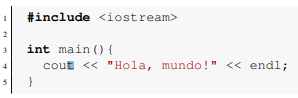
\includegraphics[width=5cm]{./Imagenes/imagen01} 
	\end{center}
	
	\item Se añade al SCV como la revisión 1 del fichero. Una vez añadido, vemos que no compila, ya que nos falta incluir el uso del espacio de nombres, así que lo modificamos:
	
	\begin{center}
	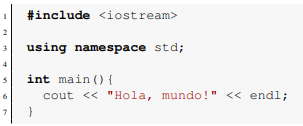
\includegraphics[width=5cm]{./Imagenes/imagen02} 
	\end{center}

	\item Se vuelve a añadir al SCV, ahora como la revisión número 2. De esta forma, se guarda el historial de las distintas modificaciones sobre un fichero, por lo que en cualquier momento podemos restaurar la revisión que queramos de un fichero.
	

\end{itemize}
\section{Actividad No 02 – Tipos de Sistemas de Control de Versiones} 

\begin{enumerate}[1.]
	\item Sistemas de Control de versiones Locales
	\\

	\begin{center}
	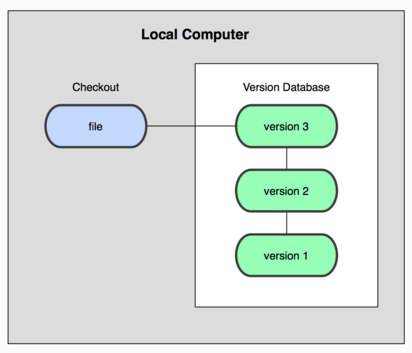
\includegraphics[width=10cm]{./Imagenes/local} 
	\end{center}

	\item Sistemas de Control de Veersiones Centralizados
	\\
	
	\begin{center}
	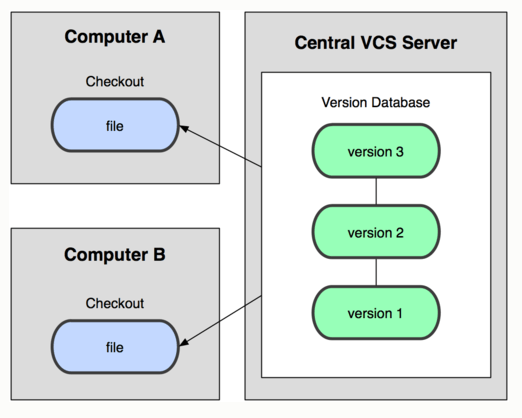
\includegraphics[width=5cm]{./Imagenes/centralizados} 
	\end{center}

	\item Sistemas de Control de Versiones Distribuidos
	\\

	\begin{center}
	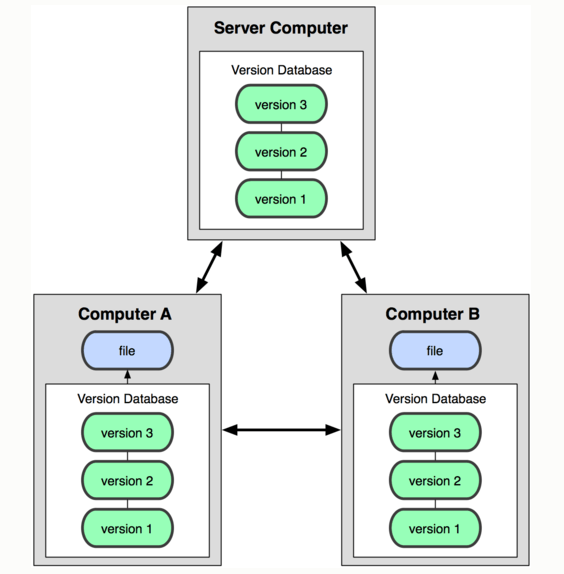
\includegraphics[width=5cm]{./Imagenes/distribuidos} 
	\end{center}

\end{enumerate}



\section{Actividad No 03 – Sistemas de Control de Versiones Libres} 
		
\begin{enumerate}[1.]
	\item CVS
	\\
	\\CVS ha estado durante mucho tiempo, y muchos desarrolladores están ya familiarizados con él. En su día fue revolucionario: fue el primer sistema de control de versiones de código abierto con acceso a redes de área amplia para desarrolladores, y el primero que ofreció ""checkouts"" anónimos de sólo lectura, los que dieron a los desarrolladores una manera fácil de implicarse en los proyectos. CVS sólo versiona ficheros, no directorios; ofrece ramificaciones, etiquetado, y un buen rendimiento en la parte del cliente, pero no maneja muy bien ficheros grandes ni ficheros binarios. Tampoco soporta cambios atómicos.
	

	\item SVK
	\\
	\\Aunque se ha construido sobre Subversion, probablemente SVK[9] se parece más a algunos de los anteriores sistemas descentralizados que a Subversión. SVK soporta desarrollo distribuido, cambios locales, mezcla sofisticada de cambios, y la habilidad de ""reflejar/clonar"" árboles desde sistemas de control de versiones que no son SVK. Vea su sitio web para más detalles.
	

	\item Mercurial
	\\
	\\Mercuria] es un sistemas de control de versiones distribuido que ofrece, entre otras cosas, "una completa ""indexación cruzada"" de ficheros y conjutos de cambios; unosprocotolos de sincronización SSH y HTTP eficientes respecto al uso de CPU y ancho de banda; una fusión arbitraria entre ramas de desarrolladores; una interfaz web autónoma integrada; [portabilidad a] UNIX, MacOS X, y Windows" y más (la anterior lista de características ha sido parafraseada del sitio web de Mercurial).
	

	\item GIT
	\\
	\\GIT es un proyecto empezado por Linus Torvalds para manejar el arbol fuente del ""kernel"" de Linux. Al principio GIT se enfocó bastante en las necesidades del desarrollo del ""kernel"", pero se ha expandido más allá que eso y ahora es usado por otros proyectos aparte del ""kernel"" de Linux. Su página web dice que está "... diseñado para manejar proyectos muy grandes eficaz y velozmente; se usa sobre todo en varios proyectos de código abierto, entre los cuales el más notable es el ""kernel"" de Linux. GIT cae en la categoría de herramientas de administración de código abierto distribuído, similar al, por ejemplo, GNU Arch o Monotone (o bitKeeper en el mundo comercial). Cada directorio de trabajo de GIT es un repositorio completo con plenas capacidades de gestión de revisiones, sin depender del acceso a la red o de un servidor central."

	\item Bazaar
	\\
	\\Bazaar está todavía en desarrollo. Será una implementación del protocolo GNU Arch, mantendrá compatibilidad con el procotolo GNU Arch a medida que evolucione, y trabajará con el proceso de la comunidad GNU Arch para cualquier cambio de protocolo que fuera requerido a favor del agrado del usuario.

\end{enumerate}








\end{document}
